\documentclass[12pt]{article}

\usepackage[a4paper, margin=1in]{geometry}
\usepackage{setspace}
\onehalfspacing
\usepackage{mathtools, amssymb, amsthm, empheq, xfrac, asymptote, hyperref, graphicx, enumitem}
\usepackage{bm}
\usepackage[dvipsnames]{xcolor}
\usepackage{ifthen}

\hypersetup{
    colorlinks=true, 
    linktoc=all,    
    linkcolor=blue, 
    urlcolor=blue
}

% commands
\newcommand{\V}{

\vspace{\baselineskip}

}
\newcommand{\comment}[1]{\textbf{\textcolor{Red}{#1}}}
% \newcommand{\image}[5][1]{
% \ifnum #1=1 
%     \begin{center}
%         \includegraphics[width=#3cm]{#2}
%     \end{center}
% \else
%     \begin{center}
%         \includegraphics[width=#3cm]{#2}
%         \includegraphics[width=#5cm]{#4}
%     \end{center}
% \fi
% }

% \setlength{\parindent}{0cm}

\title{\huge {\fontfamily{lmss}\selectfont
\textbf{IOAA Notes}}}
% \author{{\fontfamily{cmr}\selectfont
% {Andrew Liu}}}
\author{\scshape \Large Andrew Liu}
\date{{\fontfamily{cmr}\selectfont August 2022}}

\begin{document}

\maketitle

\section{Spherical Trig}

\textit{References: Roy and Clarke Chapter 9, Kartunnen Chapter 2, Carroll Ostlie Chapter 1}

\subsection{Triangle Formulas}

\begin{center}
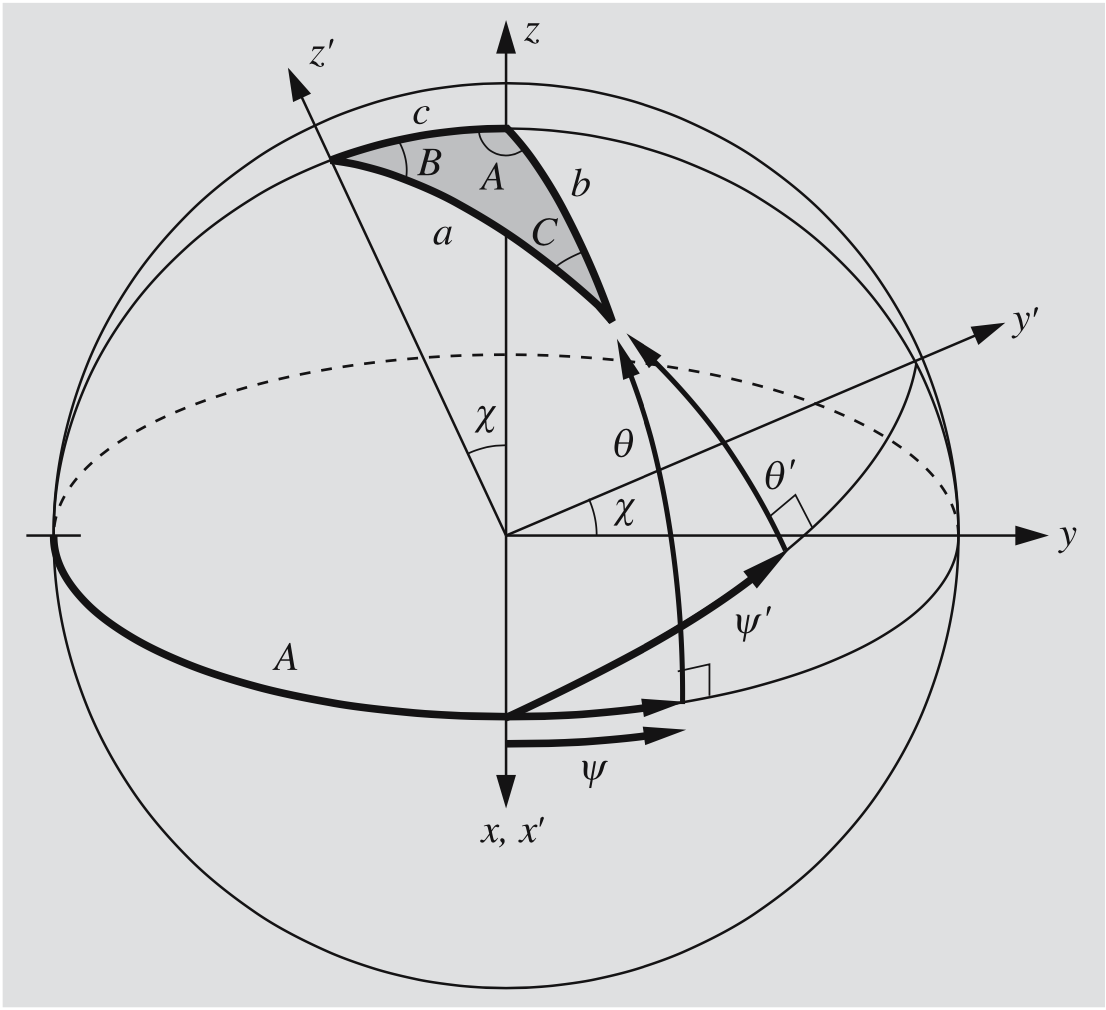
\includegraphics[width=9cm]{images/triangle.png}
\end{center}
% \image{images/triangle.png}{9}{}{}

Area:
\begin{align*}
    E = A + B + C - \pi \\
    \text{Area} = E\cdot r^2
\end{align*}

Spherical law of sines: 
\begin{equation*}
    \frac{\sin{a}}{\sin{A}} = \frac{\sin{b}}{\sin{B}} =\frac{\sin{c}}{\sin{C}}
\end{equation*}

Spherical law of cosines: 
\begin{equation*}
    \cos{a} = \cos{A}\sin{b}\sin{c}+\cos{b}\cos{c}
\end{equation*}
\begin{equation*}
    \cos{A} = \cos{a}\sin{B}\sin{C}-\cos{B}\cos{C}
\end{equation*}

Spherical law of cosines (alternate): 
\begin{equation*}
    \cos{B}\sin{a} = -\cos{A}\sin{b}\cos{c}+\cos{b}\sin{c}
\end{equation*}

Four parts formula: 
\begin{equation*}
    \cos{a}\cos{C} = \sin{a}\cot{b} - \sin{C}\cot{B}
\end{equation*}
\begin{equation*}
    \cos{A}\cos{c} = \sin{A}\cot{B} - \sin{c}\cot{b}
\end{equation*}

\subsection{Coordinate Systems}

% \image[2]{images/rah.png}{7.5}{images/conversion.png}{7.5}

\begin{center}
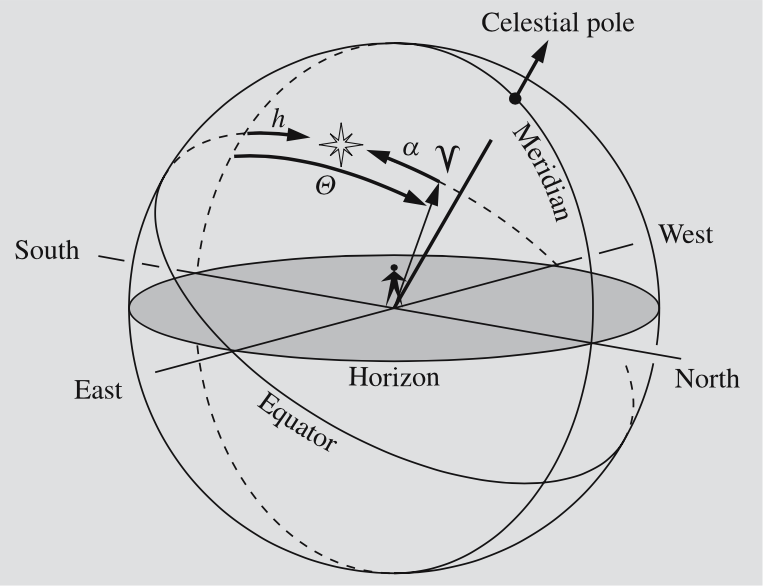
\includegraphics[width=7.5cm]{images/rah.png}
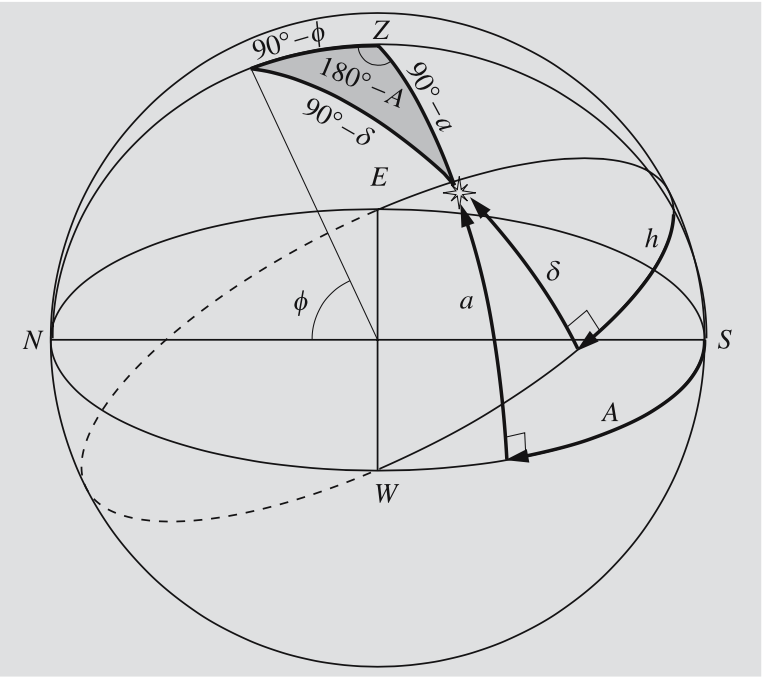
\includegraphics[width=7.5cm]{images/conversion.png}
\end{center}
%\image{images/conversion.png}

Equatorial: (Right Ascension, Declination) = $(\alpha, \delta)$

Horizontal: (Azimuth, Altitude) = $(A, a)$

Ecliptic: (Longitude, Latitude) = $(\lambda, \beta)$

Galactic: (Longitude, Latitude) = $(\ell, b)$. 

Local Sidereal Time = $\Theta = h + \alpha$. (AKA hour angle of $\Upsilon$)

\begin{itemize}
\item Azimuth $A$ measured clockwise from either the northernmost or southernmost point on observor's horizon (usually whichever is more convenient, but stick to one notation to be consistent). 

\item RA $\alpha$ measured counterclockwise from the vernal equinox ($\Upsilon$)

\item Longitude $\lambda$ measured counterclockwise from the vernal equinox ($\Upsilon$)

\item Galactic coordinates centered at the sun. Longitude $\ell$ is measured counterclockwise from the ray $\overrightarrow{\odot GC}$, where GC is the galactic center.

\item Hour angle $h$ measured clockwise from the southern meridian. Measures the time that has elapsed after an object has culminated (in the northern hemisphere).
\end{itemize}

\subsection{Timekeeping}

\textbf{Solar vs. Sidereal:} $T$ = Local Solar Time (acronym LST not to be confused with $\Theta$ = Local Sidereal Time). $\texttt{12:00}$ local solar time corresponds to the time when the sun culminates for a particular location. On March 20th, the sun aligns with the vernal equinox and thus culminates at the same time as the vernal equinox, meaning that $T = \texttt{12:00}$ and $\Theta = \texttt{0:00}$ align on this date.

Every solar day takes $24$ hours; the time between consecutive culminations of the sun takes $24$ hours. Every sidereal day takes $23$ hours $56$ minutes $4$ seconds; for any background star, the time between consecutive culminations takes $23$ hours $56$ minutes $4$ seconds. The exact conversion is 
\begin{gather*}
    24\text{ sidereal hours} = 24\cdot \left(\frac{365.25}{366.25}\right)\text{ solar hours} \\
    24\text{ solar hours} = 24\cdot \left(\frac{366.25}{365.25}\right)\text{ sidereal hours}. 
\end{gather*}
To derive this, consider that sidereal time accounts for one additional rotation of the entire earth's orbit around the sun per year, so it necessary runs faster, i.e., a sidereal hour is less than a solar hour, and any time period measured in solar time will be numerically smaller than any period measured in sidereal time.\V

To compute solar to sidereal times at specific dates, approximate 
\[
\Theta = \begin{cases}
    T + 12\text{ hr} & \text{Vernal Equinox} \\
    T + 18\text{ hr} & \text{Summer Solstice} \\
    T + 0\text{ hr} & \text{Autumnal Equinox} \\
    T + 12\text{ hr} & \text{Winter Solstice}. 
\end{cases}
\]

Then, for example, if you want to compute sidereal time on March $31$st, this corresponds to a period of $10$ solar days that passed, which is equal to $10\cdot (366.25/365.25)$ sidereal days that passed. The difference is about $40$ minutes, as we expect, since a solar day is about $4$ minutes longer than a sidereal day (in solar time). So, on March $31$st, we have $\Theta \approx T + 12\text{ hr} + 40\text{ min}$.\V

\textbf{Zero Meridian:} Greenwich, London is the $0^{\circ}$ meridian. Greenwich Mean Time (GMT), also called Universal Time (UT) is the local solar time in Greenwich and is used as the "universal" time. Greenwich Mean Sidereal Time (GMST) is the hour angle of $\Upsilon$ ignoring the effects of nutational variation (since it is measured against the background stars). Greenwich Apparent Sidireal Time (GAST) is the actual position of $\Upsilon$. Equation of the Equinoxes: 

\begin{equation*}
    \mathcal{E}_{\Upsilon} = \text{GAST} - \text{GMST}.
\end{equation*}

Convert between Greenwich and any other location with longitude $\lambda$ with: 

\begin{equation*}
    GHA\star = HA\star + \lambda,
\end{equation*}
where west $\lambda$ is positive and east $\lambda$ is negative, so that "Longitude east, Greenwich least; Longitude west, Greenwich best".\V

\textbf{Equation of Time ($\mathcal{E}$):} The mean sun (MS) is a fictitious sun that moves along the celestial equator at the rate of $(360^{\circ})/365.25\text{ days}$. The true sun ($\odot$) moves along the ecliptic at the same rate. We introduce MS for timekeeping, since the true sun does not technically have a constant angular velocity (eccentricity of orbit) and also suffers from the $23.5^{\circ}$ obliquity. Now, equation of Time ($\mathcal{E}$):

\[\mathcal{E} = \text{RAMS} - \text{RA}\odot\]

(Note that this is backwards from the Equation of the Equinoxes). Some other notes on the equation of time that are important to remember (from that one Singapore problem): 
\begin{enumerate}
    \item The equation of time can also be written as $\mathcal{E} = \text{HA}\odot - \text{HAMS}$. 
    \item Recall that timekeeping is based on the mean sun. So, whenever the equation of time is not equal to zero, $HA\odot = 0$ does not necessarily correspond to local solar time $LST = 12^{h}$.
    \item Instead, use this: $LST = HAMS \pm 12^{h} = HA\odot - \mathcal{E} \pm 12^{h}$. This is one reason why the rising time will become earlier between the vernal equinox and summer solstice, since the equation of time becomes more and more positive (for fixed hour angle, the LST is lesser). At the summer solstice, the equation of time is equal to zero, so the only reason why the sun still rises earlier at this stage is due to the fact that the sun's declination is $23.5^{\circ}$.
\end{enumerate}


\V




\textbf{Analemma}: plot with equation of time on the horizontal axis and declination on the vertical axis. See this link for a nice visual of the projection of an Analemma: \href{https://medium.com/sentinel-hub/the-shadow-of-a-celestial-dance-90968f1f42fb}{https://medium.com/sentinel-hub/the-shadow-of-a-celestial-dance-90968f1f42fb}\V

\textbf{Time Zones:} 

\begin{center}
\begin{tabular}{|c|c|}
\hline
zone & longitude \\
\hline\hline
$\pm 0$ (UTC$\pm$0) & $0^{h}30^{m}\text{W}$—$0^{h}30^{m}\text{E}$  \\
\hline
+1 (UTC-1) & $1^{h}30^{m}\text{W}$—$0^{h}30^{m}\text{W}$  \\
\hline
+2 (UTC-2) & $2^{h}30^{m}\text{W}$—$1^{h}30^{m}\text{W}$  \\
\hline
   \vdots  &\vdots  \\
\hline
+12 (UTC-12) & $12^{h}\text{W}$—$11^{h}30^{m}\text{W}$  \\
\hline
\end{tabular}
\begin{tabular}{|c|c|}
\hline
zone & longitude \\
\hline\hline
&  \\
\hline
-1 (UTC+1) & $1^{h}30^{m}\text{E}$—$0^{h}30^{m}\text{E}$  \\
\hline
-2 (UTC+2) & $2^{h}30^{m}\text{E}$—$1^{h}30^{m}\text{E}$  \\
\hline
   \vdots  &\vdots  \\
\hline
-12 (UTC+12) & $12^{h}\text{E}$—$11^{h}30^{m}\text{E}$  \\
\hline
\end{tabular}
\end{center}

% Zone $0$ is $0^{h}30^{m}W$—$0^{h}30^{m}E$. 

% Zone $+1$ (UTC-1) is $1^{h}30^{m}W$—$0^{h}30^{m}W$. Zone $+2$ (UTC-2) is $2^{h}30^{m}W$—$1^{h}30^{m}W$ ... Zone $+12$ (UTC-12) is $12^{h}W$—$11^{h}30^{m}W$.

% Zone $-1$ (UTC+1) is $1^{h}30^{m}E$—$0^{h}30^{m}E$. Zone $-2$ (UTC+2) is $2^{h}30^{m}E$—$1^{h}30^{m}E$ ... Zone $-12$ (UTC+12) is $12^{h}E$—$11^{h}30^{m}E$.

The international date line is defined by $12^{h}\text{ E/W}$. If you're travelling from east to west (in the direction from China to America) across the international date line, then you're moving from Zone $-12$ (UTC+12) to Zone $+12$ (UTC-12). To change times from Zone $-12$ to UTC, you subtract $12$ hours; to change times from UTC to Zone $+12$, you subtract $12$ hours again. In total, you lose $24$ hours. If you're travelling from west to east, you gain $24$ hours.

\newpage
\section{Cosmology}

\textit{References: Carroll Ostlie Chapter 29}\V

\textbf{Cosmological Principle}: the assumption that the expanding universe is both isotropic and homogenous.\V

\textbf{Hubble's Law:} 
\begin{equation*}
    v = H_0r.
\end{equation*}
$v$ is recessional velocity. $H_0$ is Hubble's constant. $r$ is distance. Works best for $r > 10$ Mpc, since smaller $r$ are obscured by \textit{peculiar velocities} (i.e. ``movement'' that is not caused by the expansion of spacetime, such as gravity between interacting galaxies). \V

\textbf{Co-moving coordinate and scale factor:}
\begin{equation*}
    r(t) = R(t)\cdot \varpi
\end{equation*}
$r(t)$ is the coordinate distance from the observer, $R(t)$ is the scale factor, and $\varpi$ is the \textit{co-moving coordinate}.

From cosmological time dilation and cosmological redshift, we have

\[R(z) = \frac{1}{1+z} = \frac{\Delta t_{emit}}{\Delta t_{obs}} = \frac{\lambda_{emit}}{\lambda_{obs}}.\]\V

\textbf{Deriving Friedmann:}

(this only works for a one-component universe of pressureless dust, so this technically isn't a fully complete proof)

\begin{center}
\begin{asy}
import graph; size(4cm); 
pen dps = linewidth(0.7) + fontsize(10); defaultpen(dps); /* default pen style */ 
pen dotstyle = black; /* point style */ 

draw(circle((0,0), 5), black);
draw(circle((0,0), 4.5), black);
fill(circle((0,0), 5), black+opacity(0.2));
fill(circle((0,0), 4.45), white);

draw((0,0));
draw((0,0)--4.5*dir(40), black, Arrow(5));

label("$r$", (0,0)--4.5*dir(40), dir(-50));
\end{asy}
\end{center}

Consider an expanding ring of dust with mass $m$ radially expanding with velocity $v$ (by the cosmological principle). Let $M_r$ be the total mass inside of the shell. Now, by conservation of energy,

\begin{equation}\label{eq:friedmannenergy}
\frac{1}{2}mv^{2}(t) - G\frac{M_{r}m}{r(t)} = -\frac{1}{2}mkc^{2}\varpi^{2}.
\end{equation}

Also, 

\[H(t) = \frac{v(t)}{r(t)} = \frac{v(t)}{R(t)\varpi} = \frac{d/dt(R(t))\varpi}{R(t)\varpi} = \frac{\dot{R}}{R}.\]

Plug stuff into Eq~\ref{eq:friedmannenergy} to eventually obtain:

\begin{equation*}
R^{2}\left(H^{2} - \frac{8}{3}\pi G\rho \right) = -kc^{2}.
\end{equation*}

This is equivalent to 

\begin{equation*}
\left(\frac{dR}{dt}\right)^{2} - \frac{8}{3}\pi G\rho R^{2} = -kc^{2},
\end{equation*}

which is also equivalent to 

\begin{equation*}
\left(\frac{dR}{dt}\right)^{2} - \frac{8}{3}\pi G\left(\frac{\rho_{m,0}}{R} + \frac{\rho_{rel,0}}{R^{2}} +\rho_{\Lambda,0}R^{2}\right) = -kc^{2}.
\end{equation*}


\textbf{Density:}

$\rho = \rho_{m} + \rho_{rel} + \rho_{\Lambda}$ accounts for matter (dark + baryonic = protons, neutrons), relativistic particles (photons and neutrinos), and dark energy. Relativistic density and dark energy density are taken as equivalent mass densities; that is, we let 
\[\rho_{rel} = \frac{u_{rel}}{c^{2}} = \frac{g^{*}aT^{4}}{2c^{2}} = \frac{2g^{*}\sigma T^{4}}{c^{3}},\]
where $u_{rel}$ is the energy density of relativistic particles, both photons and neutrinos. This differs from the normal energy density of blackbody radiation ($u=aT^{4}$, which only accounts for photons) by a factor of $g^{*}/2\approx 1.68$. $g^{*}$ itself is the ``effective number of degrees of freedom for relativistic particles''. Knowing what this means isn't super important but the $1.68$ figure has shown up before so just know that it exists. We also let 
\[\rho_{\Lambda} = \frac{\Lambda c^{2}}{8\pi G},\]
so that the Friedmann equation looks consistent ($8/3\pi G(\rho_{m}+\rho_{rel}) + 1/3\Lambda c^{2}$) when fully expanded.\V

\textbf{Other important equations:}

Fluid equation (for a pressureless universe, $P=0$ confirms $M_{r}$ constant in our simplified dust model):

\[\frac{d}{dt}(R^{3}\rho) = -\frac{P}{c^{2}}\frac{d(R^{3})}{dt}.\]

Acceleration equation:

\[\frac{d^{2}R}{dt^{2}} = -\frac{4}{3}\pi G\left(\rho + \frac{3P}{c^{2}}\right)R.\]

Equation of state:

\[P = wu = w\rho c^{2},\]

which along with the fluid equation implies

\[R^{3(1+w)}\rho_{x} = \text{constant} = \rho_{0,x},\]

where $w=0$ when $x$ is matter, $w=1/3$ when $x$ is radiation, and $w=-1$ when $x$ is dark energy. (for example, we know $P_{\text{rad}} = u_{\text{rad}}/3$).

We also have 

\[RT = T_{0},\]

which comes from Wien's law or from the relationship above for $x$ = radiation.\V

\textbf{Critical Density:}

When $k=0$ in the friedmann equation:

\begin{equation*}
\rho_{c}(t) = \frac{3H(t)^{2}}{8\pi G}.
\end{equation*}\V

\textbf{Density Paramters:}

\[\Omega_{x}(t) = \frac{\rho_{x}(t)}{\rho_{c}(t)} = \frac{8\pi G\rho_{x}(t)}{3H(t)^{2}}.\]

Try to remember approximately what the current density parameter values are:
\[\begin{cases}
\displaystyle \Omega_{m,0} =  \frac{8\pi G\rho_{m,0}}{3H_{0}^{2}} \approx 0.27 \\
\displaystyle \Omega_{rel,0} = \frac{16\pi Gg^{*}\sigma T_{0}^{4}}{3H_{0}^{2}c^{3}} \approx 8.24\cdot 10^{-5}\\
\displaystyle \Omega_{\Lambda,0} = \frac{\Lambda c^{2}}{3H_{0}^{2}} \approx 0.73.
\end{cases}
\]

(the current universe is dominated by dark energy, and relativistic particles are almost negligible so that $P/c^{2} << \rho$). $\Omega_{m,0}$ can be further broken down into the dark matter density parameter (roughly 0.22) and the baryonic matter density parameter (roughly 0.04). \V

Some very useful reformulations of the friedmann equation: 

\[H^{2}(1-\Omega)R^{2} = -kc^{2} = H_{0}^{2}(1-\Omega_{0}),\]

where $\Omega = \Omega_{m} + \Omega_{rel} + \Omega_{\Lambda}$. Also equivalent to

\[H = H_{0}(1+z)\left[(1+z)\Omega_{m,0} + (1+z)^{2}\Omega_{rel,0} + \frac{\Omega_{\Lambda,0}}{(1+z)^{2}} + 1-\Omega_{0}\right].\]\V

\textbf{Distances:}

\begin{itemize}
\item co-moving distance ($\varpi$): equal to current proper distance $d_{p,0}$. this definition is somewhat tautological but just accept it for now.
\item proper distance $(d_{p})$: distance between two events that occur simultaneously. In a flat universe, the proper distance is just equal to the coordinate distance, i.e., $d_{p} = \varpi/(1+z)$.
\item horizon distance $(d_{h})$: proper distance to the farthest observable point in the universe (the particle horizon).
\item luminosity distance $(d_{L})$: measured flux $F = L/(4\pi d_{L}^{2}) = L/(4\pi \varpi^{2} (1+z)^{2})$, so $d_{L} = \varpi (1+z)$. Oftentimes solve for luminosity distance using distance modulus (i.e. given apparent and absolute magnitude) and need to convert to proper distance *at the present time* using $d_L = \varpi (1+z) = d_{p,0} (1+z)$. 
\item angular distance $(d_{A})$: $d_{A} = D/\theta = \varpi/(1+z)$.
\end{itemize}

Example calculation of $\varpi$, $d_{p}$, and $d_{h}$ for a flat, one-component universe of pressureless dust: 

\begin{center}
\includegraphics[width=6cm]{images/varpi-1.png}
\includegraphics[width=6cm]{images/varpi-2.png}
\end{center}
% \image[2]{images/varpi-1.png}{6}{images/varpi-2.png}{6}

\newpage
\section{Radio Astronomy}

\textit{References: Carroll Ostlie Chapters 3 and 9, Karttunen Chapter 4}\newline
\url{https://lweb.cfa.harvard.edu/~eprice/files/notes00.pdf}

\subsection{Terms:}
\begin{itemize}
\item \textbf{Itensity} ($I$): measured in $Wm^{-2}\text{ Sterad}^{-1}$. This refers to total intensity. Monochromatic intensity (specific intensity) $I_\nu$ has units of $Wm^{-2}\text{ Sterad}^{-1}Hz^{-1}$, and is formally defined as follows: $E_{\nu}d\nu = I_{\nu} d\nu dA d\Omega dt$ (the quantity $E_{\nu}d\nu$ is the amount of energy that exists between the frequencies $\nu$ and $\nu + d\nu$). $I = \int I_{\nu}d\nu$.
\item \textbf{Flux} ($F$): (technically Flux Density) measured in $Wm^{-2}$, is the amount of energy per unit time from a radiation source that passes through some unit surface $S$. Alternatively, this can be thought of as the integral of Intensity through some solid angle. Monochromatic flux density (specific radiative flux), has units $Wm^{-2}Hz^{-1}$ (=$10^{26}$ Janskys) can be expressed as follows: $F_{\nu} d\nu = \int_S \frac{E_{\nu}d\nu}{dt dA} = \int_S I_{\nu}d\nu \cos{\theta} d\Omega$. $F = \int F_{\nu}d\nu$, which is also equal to $\int_S I\cos{\theta}d\Omega$ so long as the intensity is received uniformly through all wavelengths (unrealistic).
\item \textbf{Luminosity} ($L$): measured in $W$, this quantity represents the total energy per unit time emitted through some surface area $A$ and solid angle. This can also be thought of as the integral of Flux density through an entire receiving surface area. Monochromatic luminosity (specific luminosity) has units of $WHz^{-1}$ and is expressed as follows: $L_{\nu}d\nu = \int_A F_{\nu}d\nu$. Then, $L = \int L_{\nu}d\nu$.
\item \textbf{Energy Density of Radiation} ($u$): Measured in J/m$^3$. See below for derivation of the formula.
\item \textbf{Surface Brightness} ($\mu$): See below.
\end{itemize}

\textbf{Surface Brightness:}

SB is a measure of flux density per unit solid angle. Typically given in units of mag/arcsec$^2$ (MPSAS -- magnitudes per square arcseconds). Given SB = $\mu$, and an object with area $A$ in units of arcsec$^2$, its apparent magnitude $m$ is given by:
\[m - \mu = -2.5\log{A}.\]
Intuitively, $\mu$ is the magnitude of the object when $A = 1\text{arcsec}^2$, so the "$\log{A}$" term just represents the ratio of fluxes in an object with area $A$. Recall that flux is equal to the amount of energy (from photons) collected per unit area of a detector on earth -- the amount of energy collected is proportional to the area of the sky that the object takes up.

Surface brightness is invariant of distance. Flux density and the solid angle both drop off with distance squared ($\Omega = A/r^2$).

\subsection{Useful Derivations / Formulas:}

% \image[2]{images/intensity.png}{6}{images/fluxdistance.png}{6}
\begin{center}
    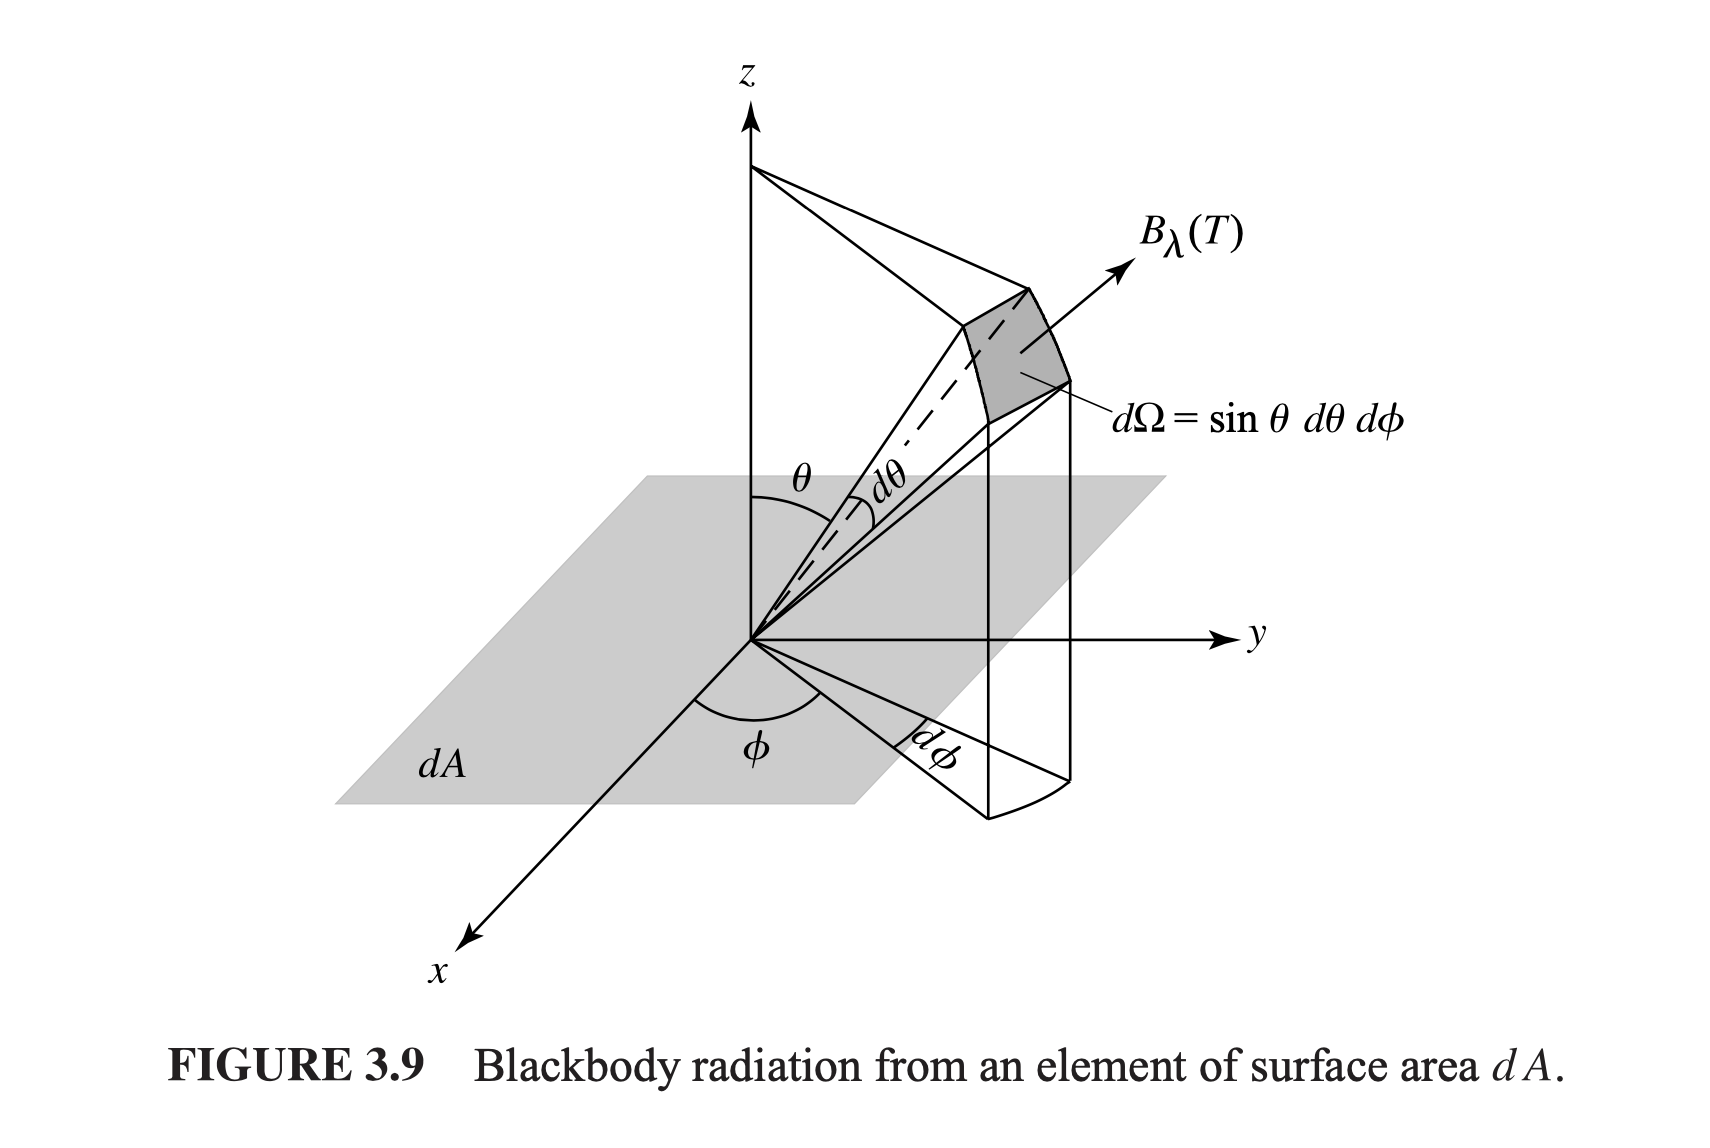
\includegraphics[width=13cm]{images/intensity.png}
    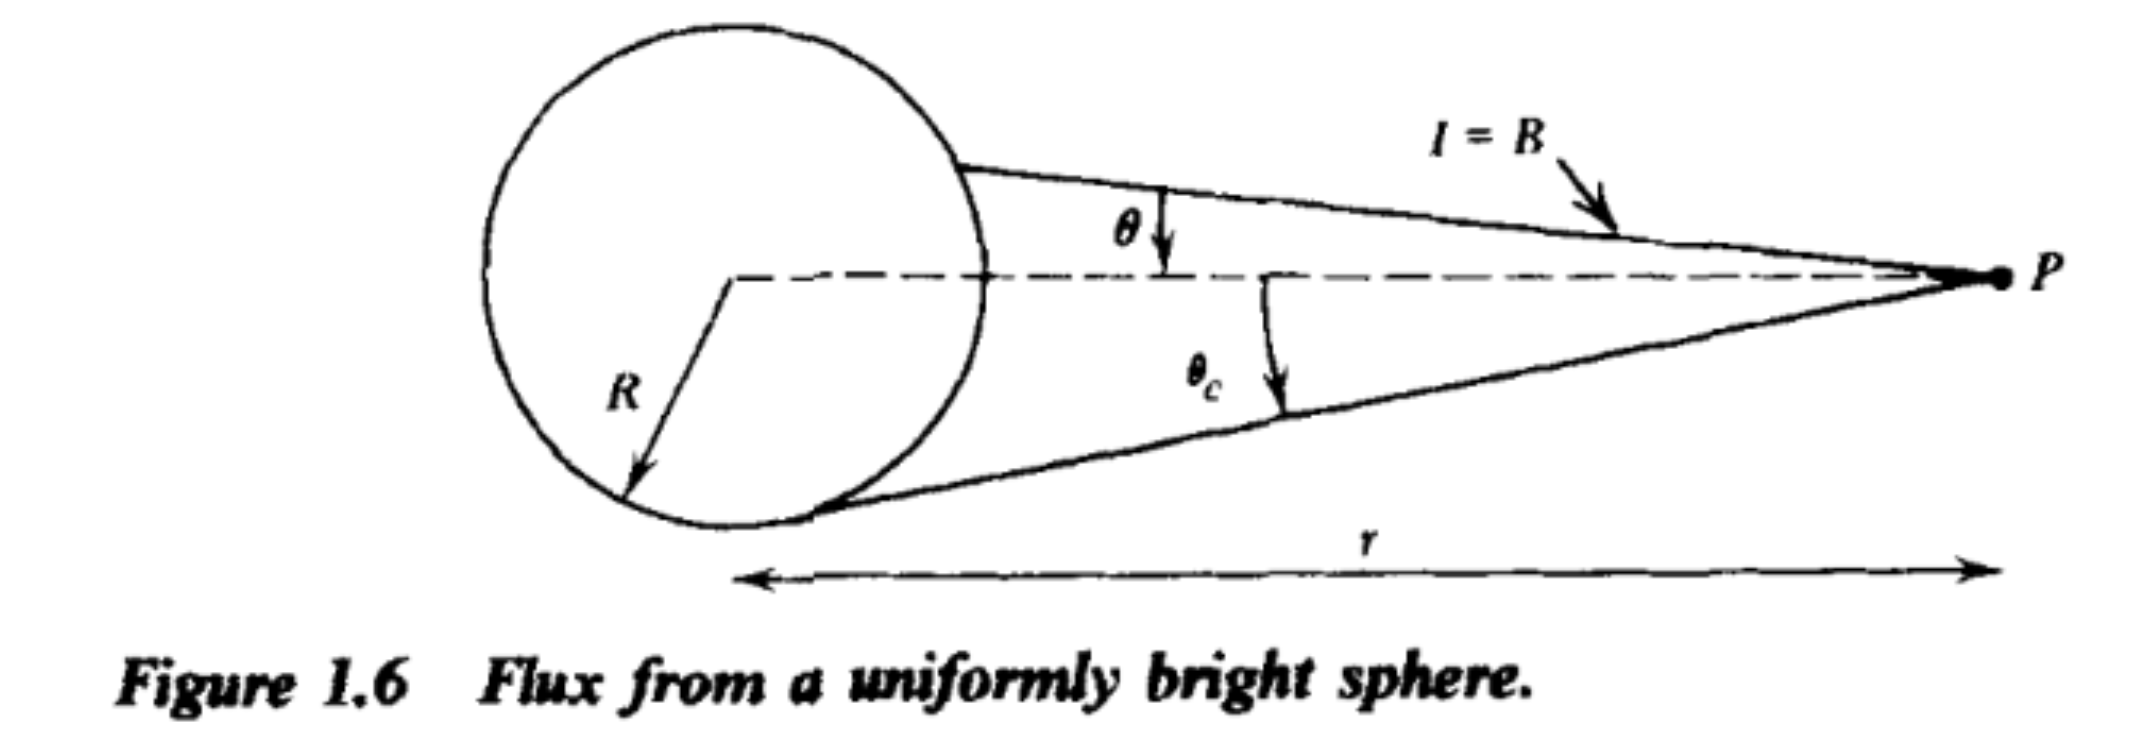
\includegraphics[width=13cm]{images/fluxdistance.png}
\end{center}

\textbf{Flux vs. Intensity:}\newline
The top image depicts a monochromatic intensity element for a blackbody (notated with the planck function $B_{\lambda}(T)$) passing through a sheet $dA$. To calculate the received flux at a distance $r$, given that the blackbody has radius $R$, we can integrate according to the bottom image:
\begin{align*}
F_{\nu}d\nu &= \int_S I_{\nu}d\nu\cos{\theta}d\omega \\
&= I_{\nu}d\nu \int_{\phi = 0}^{2\pi}\int_{\theta = 0}^{\theta_c}\cos{\theta}\sin{\theta}\mathrm{d}\phi \mathrm{d}\theta \\
&= 2\pi I_{\nu}d\nu\int_{0}^{\theta_c}1/2\cdot \sin{2\theta}\mathrm{d}\theta \\
&= \pi I_{\nu}d\nu (1-\cos^2{\theta_c}) = \pi I_{\nu}d\nu \sin^2{\theta_c}.
\end{align*}

Assuming that the radiation is uniform across all wavelengths, this implies that $F = \pi I \sin^2\theta_c = \pi I (R/r)^2 \approx I\Omega$ (when given the angular diameter of a faraway object this approximation is usually pretty good). Note that when $r=R$ we have $F = \pi I$.\V

\textbf{Planck Functions:}

\[B_{\lambda}(T) = \frac{2hc^2/\lambda^5}{e^{hc/\lambda kT} - 1}.\]
\[B_{\nu}(T) = \frac{2h\nu^3/c^2}{e^{h\nu/kT} - 1}.\]

Rayleigh Jeans approximation (for $\nu$ small):
\[B_{\nu}(T) \approx \frac{2\nu^2}{c^2}kT.\]

\textbf{Total intensity:}
\[I = \int_0^{\infty} B_{\lambda}(T)\mathrm{d}\lambda =  \int_0^{\infty} B_{\nu}(T)\mathrm{d}\nu = F/\pi.\]

By design, $B_{\lambda}(T)d\lambda = -B_{\nu}(T)d\nu$, where $d\lambda = -c/\nu^2 d\nu$. Performing this integral yields:

\[F = \left(\frac{2\pi^5 k^4}{15c^2 h^3}\right)T^4 = \sigma T^4.\]

\textbf{Energy Density:}

"Capture energy in a cylindrical trap". 

\begin{center}
    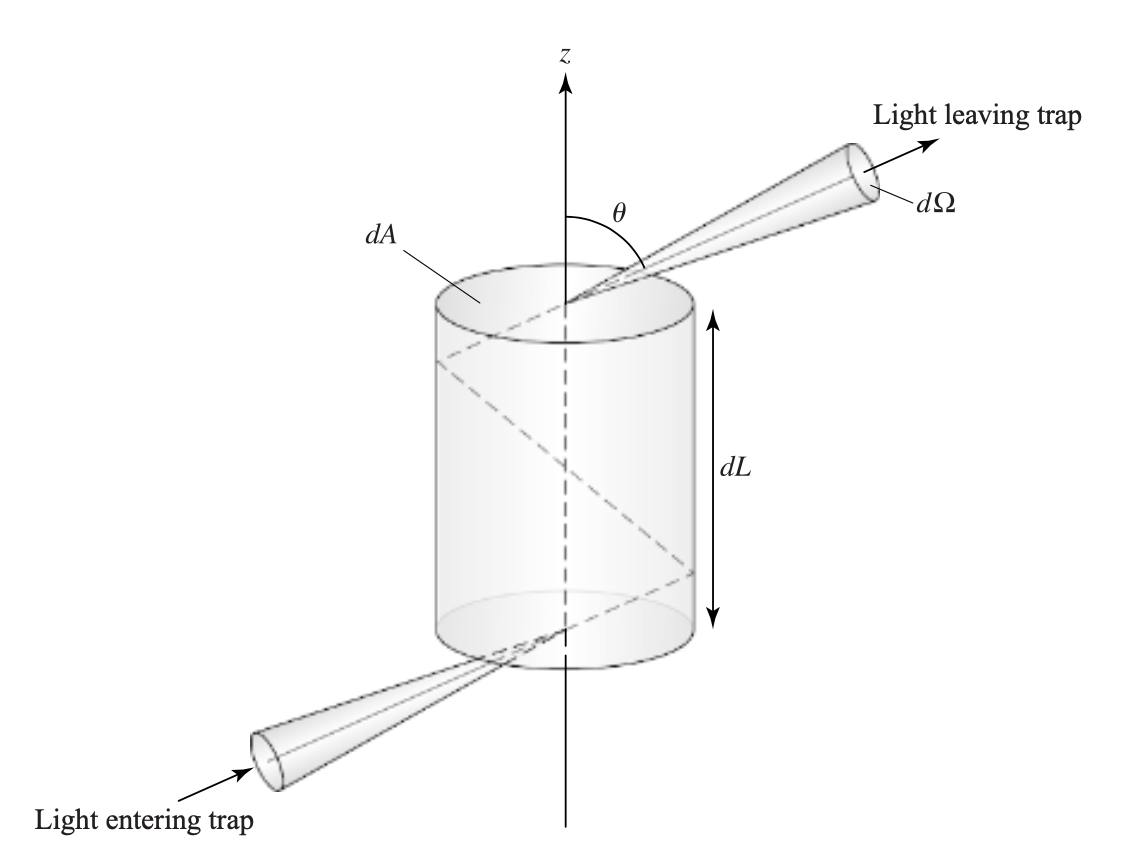
\includegraphics[width=10cm]{images/energydensity.png}
\end{center}

\[E_{\nu}d\nu = I_{\nu}d\nu dA\cos{\theta}dtd\Omega = I_{\nu}d\nu dA\cos{\theta}\left(\frac{dL}{c\cdot \cos{\theta}}\right)d\Omega\]

The first $\cos{\theta}$ comes from the fact that energy is diminished because of the angle at which the light enters the trap. However, this is ultimately negated by the fact that the light spends more time inside of the trap by a factor of $1/\cos{\theta}$. 

Now, let $du_{\nu}d\nu$ be a specific energy density element, the first differential with respect to our solid angle. 

\[du_{\nu}d\nu = \frac{E_{\nu}d\nu}{dV} = I_{\nu}d\nu d\Omega \cdot 1/c.\]

Assuming that intensity is the same in every direction, integrating over every solid angle thus gives: 
\[u_{\nu}d\nu = \frac{4\pi}{c}I_{\nu}d\nu.\]

Finally, integrating over all wavelengths: 
\[u = \frac{4\pi}{c}\int I_{\nu}d\nu = \frac{4\sigma T^4}{c} = aT^4,\]

where $a \equiv 4\sigma/c$ is the radiation constant.\V

\textbf{Radiation Pressure:}

Let $dp_{\nu}d\nu$ equal the total momentum contained in an incident cone of light to a wall, with solid angle $d\Omega$ (frequencies between $\nu$ and $\nu + d\nu$). Let $dP_{\nu}d_{\nu}$ be the total pressure exerted by this cone of light. Then, 
\[dp_{\nu}d\nu = \left(\frac{2E_{\nu}\cos{\theta}}{c}\right)d\nu.\]

Thus, 

\[dP_{\nu}d\nu = \frac{dp_{\nu}d\nu/dt}{dA} = I_{\nu}d\nu\cdot \frac{2}{c}\cos^2{\theta}d\Omega.\]

Integrating everything gives $P = u/3$. When not accounting for all incidental angles, the factor of $\cos^2{\theta}$ can be dropped (i.e. just a cone of light incident perpendicular to our wall). Integration in this case leads to $P = u$. The factor of three that is present in the original derivation can be thought of approximately due to the symmetries in each of the three dimensions.

Things can also be framed with respect to the time averaged Poynting vector $\langle S\rangle$. For absorption:

\[F_{\text{rad}} = \frac{\langle S\rangle A}{c}\cos{\theta} \implies P_{\text{rad}} = \frac{\langle S\rangle}{c} = u.\]

For reflection, every of the above quantities is doubled.

\newpage
\section{Celestial Mechanics}

\textit{References: Carroll Ostlie Chapter 2, Karttunen Chapter 6}

\subsection{Two-body System}

\[\mu = \frac{m_1m_2}{m_1 + m_2}, M = m_1+m_2\]
\[\mathbf{r_1} = \frac{\mu}{m_1}\mathbf{r}, \mathbf{r_2} = \frac{\mu}{m_2}\mathbf{r}, \mathbf{v_1} = \frac{\mu}{m_1}\mathbf{v}, \mathbf{v_2} = \frac{\mu}{m_2}\mathbf{v}.\]

\textbf{Total Energy:}
\[E = \frac{1}{2}m_1v_1^2 + \frac{1}{2}m_2v_2^2 - \frac{Gm_1m_2}{r} =  \frac{1}{2}\mu v^2 - G\frac{M\mu}{r}.\]

\textbf{Total Angular Momentum:}
\[\mathbf{L} = m_1\mathbf{r_1}\times \mathbf{v_1} + m_2\mathbf{r_2}\times\mathbf{v_2} = \mu \mathbf{r}\times \mathbf{v} = \mathbf{r}\times \mathbf{p}.\]
\[L = \mu\sqrt{GMa(1-e^2)}.\]

\textbf{Other formulas:}
\[v_p = \sqrt{\frac{GM(1+e)}{a(1-e)}}, v_a = \sqrt{\frac{GM(1-e)}{a(1+e)}}.\]
\[dA = \frac{1}{2}(r\times dr) = \frac{1}{2}(r\times vdt) = \frac{L}{2\mu}dt.\]
\[dA = \frac{1}{2}r^2d\theta.\]
\[d\mathbf{L}/dt = (d\mathbf{r}/dt\times \mathbf{p}) + (\mathbf{r}\times d\mathbf{p}/dt) = \mathbf{v}\times \mu \mathbf{v} + \mathbf{r}\times \mathbf{F} = 0.\]

\subsection{Conics}

General polar form of orbital equations: 
\[r = \frac{p}{1 + e\cos{\theta}}.\]

\begin{itemize}
    \item Circle: Constant radius, $e=0$.
    \[r = p.\]
    \item Ellipse: $p = b^2/a = a(1-e^2)$, $0 < e < 1$.
    \[r = \frac{a(1-e^2)}{1 + e\cos{\theta}}.\]
    \item Parabola: $p = 2r_p$, $r_p=$ perihelion distance. $e=1$.
    \[r = \frac{2r_p}{1+\cos{\theta}}.\]
    \item Hyperbola: $p = b^2/a = a(e^2-1)$, $e > 1$. 
    \[r = \frac{a(e^2-1)}{1+e\cos{\theta}}.\]
\end{itemize}

\newpage
\section{Atmosphere}

\textit{References: Carroll Ostlie Chapter 9}\V

\textbf{Mean free path} ($\ell$): average distance that molecule travels between collisions. 

\[\ell = \frac{1}{n\sigma} = \frac{1}{\rho \kappa}.\]

\begin{itemize}
    \item $n = \rho / m$ is the number density of the molecule. For a hydrogen atom, $m = m_h$. 
    \item $\sigma = \pi(2r)^2$ is the collision cross section. For a hydrogen atom, $r = a_0$ is the Bohr radius. 
    \item $\rho$ is the mass density of the molecule in the gas.
    \item $\kappa$ is called the absorption coefficient, also known as opacity. 
\end{itemize}

The left hand expression can be derived using the cylinder method. If $vt$ represents the total distance travelled by the collision cross section in time $t$, and $vtn\sigma$ represents the total number of stationary particles sweeped by the collision cross section, so dividing the two quantities gives us our desired value for $\ell$.\V

\textbf{Length of random walk} (d): 

Consider a random walk of a photon travelling through a stellar atmosphere with $N$ steps. Then, the net displacement vector is given by: 

\[\mathbf{d} = \sum_{i=1}^N \bm{\ell}_i.\]

To compute the magnitude of $\mathbf{d}$:

\[\mathbf{d}\cdot \mathbf{d} = \sum_{i=1}^{N}\sum_{j=1}^N \bm{\ell}_i\cdot \bm{\ell}_j.\]

This implies

\[d^2 = N\ell^2 + 2\ell^2\sum_{i=1}^{N}\sum_{j=i+1}^{N}\cos{\theta_{ij}}.\]

Over a long period of time, this gives us $d\approx \ell \sqrt{N}$. The number of steps required to get to escape to the surface is then approximately equal to \[N \approx \left(\frac{d_{\text{surface}}}{\ell}\right)^2 = \left(\frac{\tau_{\lambda} \ell}{\ell}\right)^2 = \tau_{\lambda}^2. \]

\V

\textbf{Optical Depth} ($\tau_{\lambda}$): 
The change in intensity of a light ray as it travels through a vacuum is zero. The change in intensity of a light ray as it travels through a gas is proportional to the density of the gas, $\rho$, the current intensity of the light ray, $I_{\lambda}$, and the distance travelled, $ds$.
\[dI_{\lambda} = -\kappa_{\lambda}\rho I_{\lambda}ds.\]

Now we define optical depth:
\[d\tau_{\lambda} = -\kappa_{\lambda}\rho ds,\]

which can be thought of loosely as the number of mean free paths required for a particle to escape the atmosphere, at any given depth. $\tau_{\lambda} = 2/3$ is generally the limit in terms of the depth at which we are able to see into any given atmosphere.

Consider a light ray observed on Earth from an angle $\theta$ from the vertical. Let $\tau_{\lambda, 0}$ be the optical depth from any light ray observed perpendicular to the earth. Then: 

\[d\tau_{\lambda} = -\kappa_{\lambda}\rho ds = -\kappa_{\lambda}\rho dz \sec{\theta} = d\tau_{\lambda, 0}\sec{\theta}.\]

Integrating the opacity equation, we get 
$I_{\lambda} = I_{\lambda,0}e^{-\tau_{\lambda, 0}\sec{\theta}}$, where $I_{\lambda}$ is the observed intensity, and $I_{\lambda,0}$ is the intensity of the light ray before entering earth's atmosphere.

\newpage
\section{Thermodynamics}






\end{document}
